\documentclass[12pt,a4paper]{article}
\usepackage[utf8]{inputenc}
\usepackage[spanish]{babel}
\usepackage{amsmath}
\usepackage{amsfonts}
\usepackage{amssymb}
\usepackage{graphicx}
\usepackage[left=2cm,right=2cm,top=2cm,bottom=2cm]{geometry}

%--------------------------------------------------------%
% Paquetes usados sólo para esta relación de ejercicios  %
%--------------------------------------------------------%

\usepackage{enumitem}
\usepackage{algorithm}
\usepackage{algorithmic}
\usepackage[hidelinks]{hyperref}

\usepackage{subcaption}


\author{Ignacio Aguilera Martos}
\title{Práctica 3 \\ Visión por Computador}
\date{22 de Diciembre de 2018}

\setlength{\parindent}{0cm}


\begin{document}
	\maketitle

	\tableofcontents

	\newpage

	%p 56

%	\framebox[16cm][c]{\LaTeX}

\section{Ejercicio 1}

Emparejamiento de descriptores.
\begin{itemize}
  \item Mirar las imágenes en imagenesIR.rar y elegir parejas de imágenes que tengan partes de escena comunes. Haciendo uso de una máscara binaria o de las funciones extractRegion() y clickAndDraw(), seleccionar una región en la primera imagen que esté presente en la segunda imagen. Para ello sólo hay que fijar los vértices de un polígono que contenga a la región.
  \item Extraiga los puntos SIFT contenidos en la región seleccionada de la primera imagen y calcule las correspondencias con todos los puntos SIFT de la segunda imagen (ayuda: use el concepto de máscara con el parámetro mask)
  \item Pinte las correspondencias encontradas sobre las imágenes.
  \item Jugar con distintas parejas de imágenes, valorar las correspondencias correctas obtenidas y extraer conclusiones respecto a la utilidad de esta aproximación de recuperación de regiones/objetos de interés a partir de descriptores de una región.
\end{itemize}

\subsection*{\underline{Solución}}

Las parejas que he escogido han sido dos para ejemplificar el buen comportamiento cuando las imágenes son similares entre sí y otra en la que el reconocimiento no es tan bueno.

\vspace{10px}

Las parejas escogidas son:

\begin{figure}[H]
  \centering
    \begin{subfigure}{0.45\textwidth}
      
\includegraphics[scale=0.33]{./Imagenes/1.png}
    \end{subfigure}
    \begin{subfigure}{0.45\textwidth}
      
\includegraphics[scale=0.33]{./Imagenes/4.png}
    \end{subfigure}
    \caption{Imágenes 1 y 4}
\end{figure}

\begin{figure}[H]
  \centering
    \begin{subfigure}{0.45\textwidth}
      
\includegraphics[scale=0.33]{./Imagenes/23.png}
    \end{subfigure}
    \begin{subfigure}{0.45\textwidth}
      
\includegraphics[scale=0.33]{./Imagenes/24.png}
    \end{subfigure}
    \caption{Imágenes 23 y 24}
\end{figure}

\begin{figure}[H]
  \centering
    \begin{subfigure}{0.45\textwidth}
      
\includegraphics[scale=0.33]{./Imagenes/91.png}
    \end{subfigure}
    \begin{subfigure}{0.45\textwidth}
      
\includegraphics[scale=0.33]{./Imagenes/92.png}
    \end{subfigure}
    \caption{Imágenes 91 y 92}
\end{figure}

La forma de proceder es, mostrar la imagen para que se pueda seleccionar la región de la misma que se desee. Esta región es diferenciada del resto mediante una máscara. La construcción de dicha máscara se hace tomando los puntos que determinan el polígono de la región y, mediante la función fillConvexPoly se rellena esta área a blanco, esto es $(255,255,255)$. Tras esto sólo tenemos que crear una matriz de ceros del mismo tamaño que la imagen y, en dichos puntos poner el valor 1. Con esto tendríamos una máscara que podemos aplicar a la función detectAndCompute para hallar los keypoints y descriptores sólo de la región que engloba el polígono.

\vspace{10px}

Hay que tener en cuenta que la detección puede ser buena si realmente hay un parecido importante entre la región que hemos seleccionado y alguna región de la imagen con la que queremos emparejar. Por ejemplo veamos los dos primeros ejemplos y analicémoslos.

\begin{figure}[H]
  \centering
  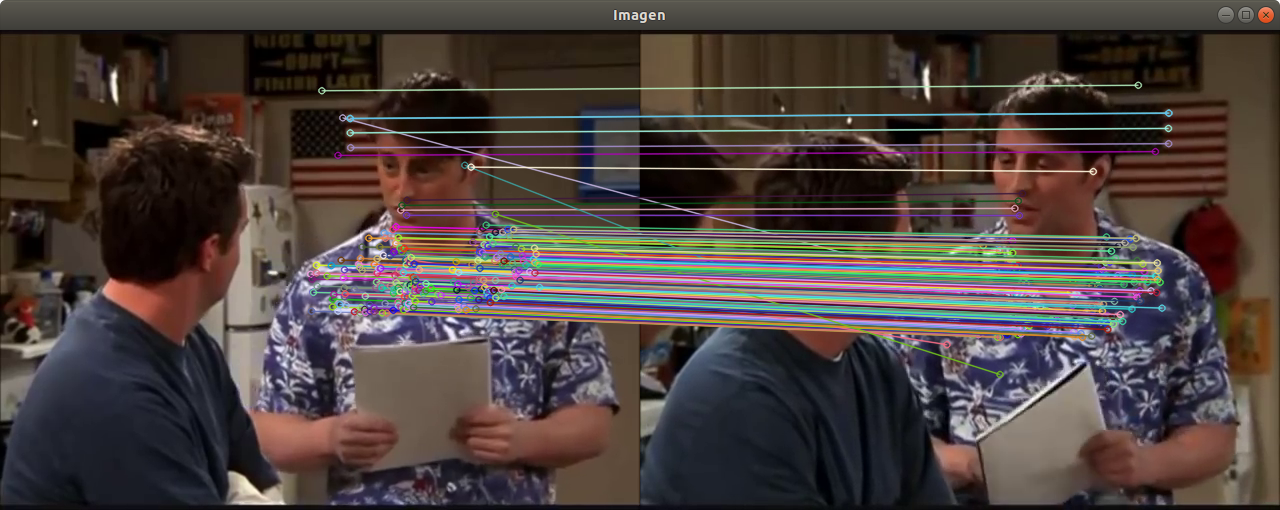
\includegraphics[scale=0.35]{./Imagenes/Ejercicio1-1.png}
  \caption{Emparejamiento con las imágenes 91 y 92}
\end{figure}

\begin{figure}[H]
  \centering
  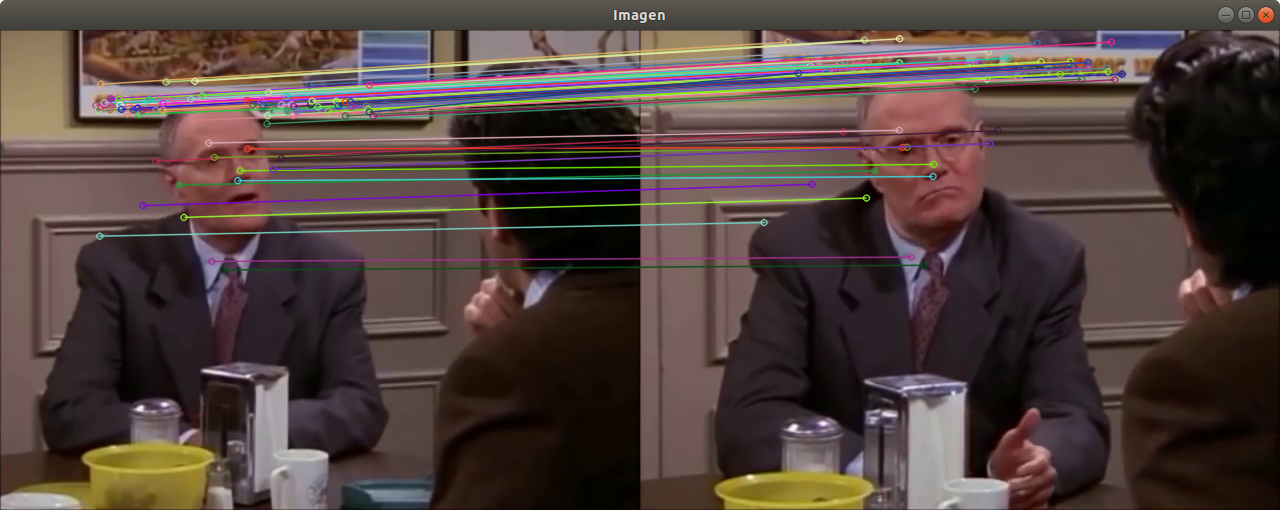
\includegraphics[scale=0.35]{./Imagenes/Ejercicio1-2.png}
  \caption{Emparejamiento con las imágenes 23 y 24}
\end{figure}

Como podemos ver claramente en estas dos imágenes el emparejamiento es muy bueno puesto que los parecidos entre las dos es muy alto. Es prácticamente la misma cara con la misma escena y el mismo fondo, por lo que no sólo se empareja la cara o la figura de la persona, si no, también el fondo como en el segundo de los casos con el cuadro que se encuentra tras la persona.

\vspace{10px}

Cabe decir que esta detección puede variar enormemente como en el siguiente caso paradigmático.

\begin{figure}[H]
  \centering
  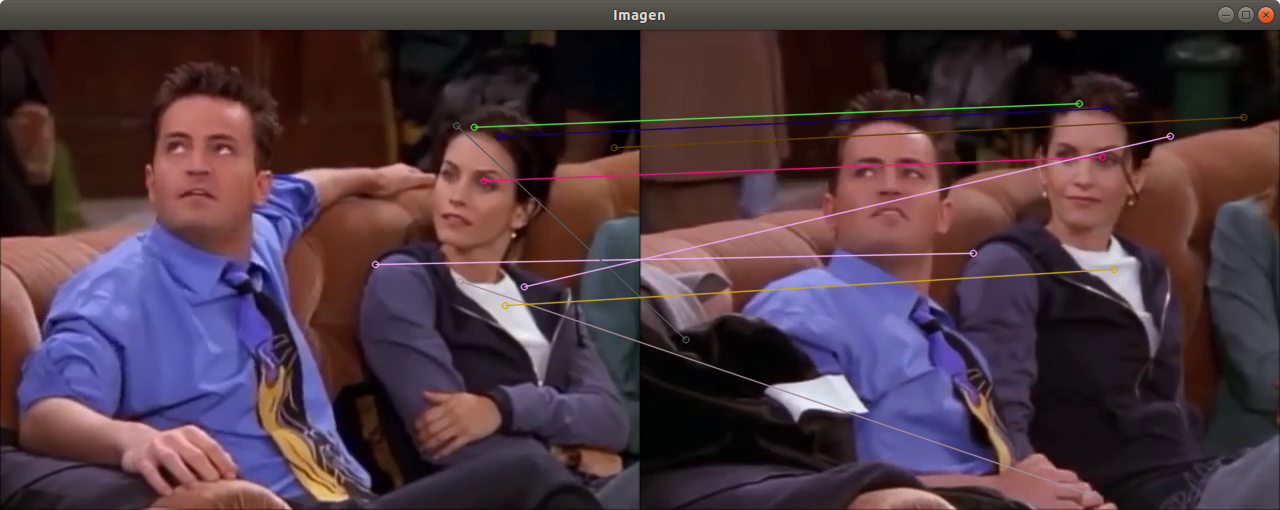
\includegraphics[scale=0.35]{./Imagenes/Ejercicio1-3.png}
  \caption{Emparejamiento con las imágenes 1 y 4}
\end{figure}

En este caso podemos ver que la detección es mucho peor pero analicemos por qué. Realmente si observamos cada uno de los keypoints como se relacionan con la imagen de la derecha vemos que el emparejamiento de los mismos es razonable salvo dos de ellos, pero este emparejamiento es muy pobre porque no hemos obtenido suficientes puntos de interés en la región como para obtener un emparejamiento sólido como en los dos primeros casos.

\vspace{10px}

Ahora bien, podemos tomar también dos imágenes de una escena que compartan una figura como por ejemplo la mujer que se enseña en las imágenes siguientes:

\begin{figure}[H]
  \centering
    \begin{subfigure}{0.45\textwidth}
      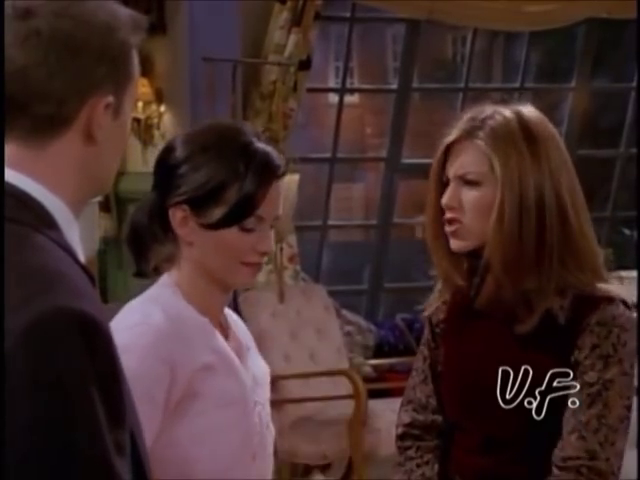
\includegraphics[scale=0.33]{./Imagenes/142.png}
    \end{subfigure}
    \begin{subfigure}{0.45\textwidth}
      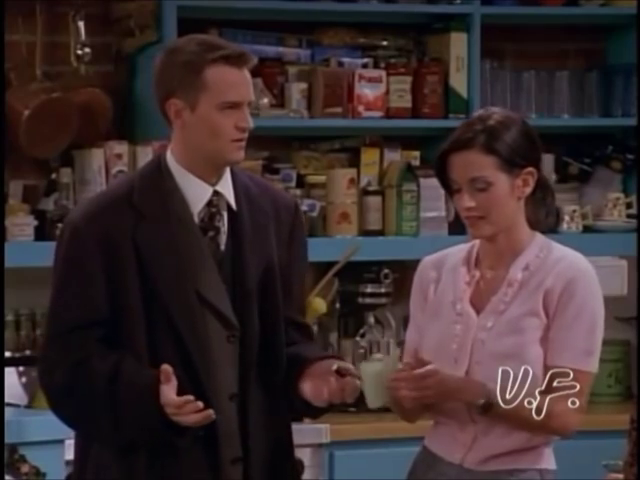
\includegraphics[scale=0.33]{./Imagenes/143.png}
    \end{subfigure}
    \caption{Imágenes 142 y 143}
\end{figure}

Veamos que la detección en este caso no es satisfactoria cuando tomamos el polígono sobre la figura de la mujer.

\begin{figure}[H]
  \centering
  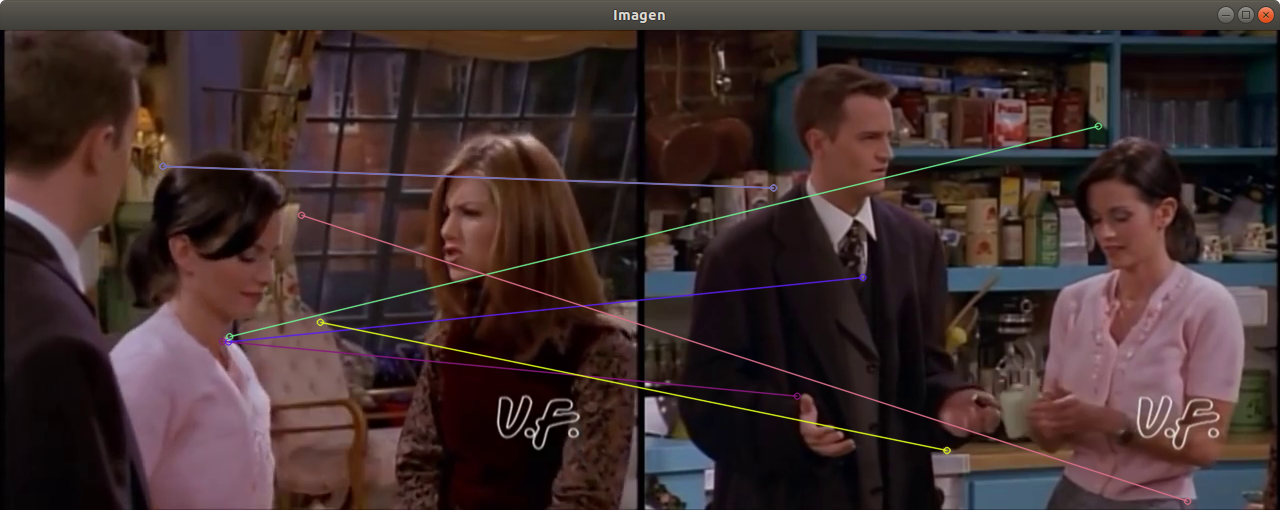
\includegraphics[scale=0.35]{./Imagenes/Ejercicio1-4.png}
  \caption{Emparejamiento con las imágenes 142 y 143}
\end{figure}

Como podemos observar nosotros estamos viendo que la mujer que aparece en la imagen de la izquierda es la misma que en la parte de la derecha pero la detección asigna los puntos de forma completamente errónea con respecto a la figura de la misma. Este fallo viene sobre todo dado porque el fondo de las imágenes es completamente distinto y por tanto, los puntos de interés tomados (que hacen el contraste en este caso de la mujer con el fondo) se ven completamente irrelevantes con respecto a la correlación que hace de los mismos.

\vspace{10px}

Por lo tanto podemos concluir que el uso de esta aproximación a la recuperación de regiones de interés a partir de descriptores de una región es en general útil pero conociendo las limitaciones, tanto de la obtención de un número de puntos de interés demasiado bajo como de el emparejamiento erróneo que pueda realizar la misma con otra imagen en la que sí comparten una región pero el fondo o la iluminación han cambiado y no se perciben las regiones como similares.

\section{Ejercicio 2}
Recuperación de Imágenes
\begin{itemize}
  \item Implementar un modelo de índice invertido+bolsa de palabras para las imágenes dadas en imagenesIR.rar usando el vocabulario dado en kmeanscenters2000.pkl
  \item Verificar que el modelo construido para cada imagen permite recuperar imágenes de la misma escena cuando la comparamos al resto de imágenes de la base de datos.
  \item Elegir dos imágenes-pregunta en las que se ponga de manifiesto que el modelo usado es realmente muy efectivo para extraer sus semejantes y elegir otra imagen-pregunta en la que se muestre que el modelo puede realmente fallar. Para ello muestre las cinco imágenes más semejantes de cada una de las imágenes-pregunta seleccionadas usando como medida de distancia el producto escalar normalizado de sus vectores de bolsa de palabras.
  \item Explicar qué conclusiones obtiene de este experimento.
\end{itemize}

\subsection*{\underline{Solución}}

El primer paso en la realización del ejercicio es obtener la frecuencia de aparición de cada centroide en cada imagen. Para ello lo que tenemos que hacer es, dada una imagen, calcularle los descriptores y calcular para cada uno de ellos cuál es el elemento de kmeanscenters2000.pkl que está más cercano. Esta intormación la he guardado en un diccionario de Python de forma que la clave sería el índice correspondiente al centroide y el valor el número de veces que aparece dicho centroide. Con esta información para cada una de las imágenes tendremos un vector de histogramas.

\vspace{10px}

Si queremos elaborar un modelo de índice invertido tenemos que pensar que ahora queremos guardar para cada centroide en qué imágenes aparece. Para obtener esto tenemos que ir recorriendo la estructura de histogramas y para cada centroide comprobar si aparece en el histograma correspondiente a dicha imagen. De esta forma acabamos con una estructura en la que para cada índice de centroides tenemos los índices correspondientes a las imágenes en las que al menos un descriptor tiene a dicho centroide como el más cercano.

\vspace{10px}

Para el estudio de la similitud de dos imágenes vamos a emplear la siguiente medida:

$$<u,v> = |u|\cdot |v|\cdot \cos{\theta}$$

Lo que estamos empleando no es más que el producto escalar de dichos vectores. Hay que tener en cuenta que los histogramas que he mencionado anteriormente pueden verse también como vectores, donde tienen en cada posición un cero si dicho centroide no es el más cercano para ningún descriptor o un número mayor que cero que representa cuántas veces ha sido el más cercano para algún descriptor de la imagen. Estos vectores normalizados son los que vamos a emplear para estudiar si dos imágenes son similares.

\vspace{10px}

Como he dicho los vectores están normalizados, por lo que la norma de los mismos es 1 y por tanto nuestra medida de similitud nos queda:

$$<u,v> = \cos{\theta}$$

O lo que es lo mismo, un valor entre -1 y 1. En nuestro caso queremos que los vectores sean lo más parecidos entre sí, esto es que el ángulo que formen sea lo más cercano a cero y se traduce por tanto en que el producto escalar esté lo más próximo a 1.

\vspace{10px}

Una vez tenemos todo este modelo de similitudes, veamos los resultados obtenidos con las siguientes imágenes pregunta:

\begin{figure}[H]
  \centering
  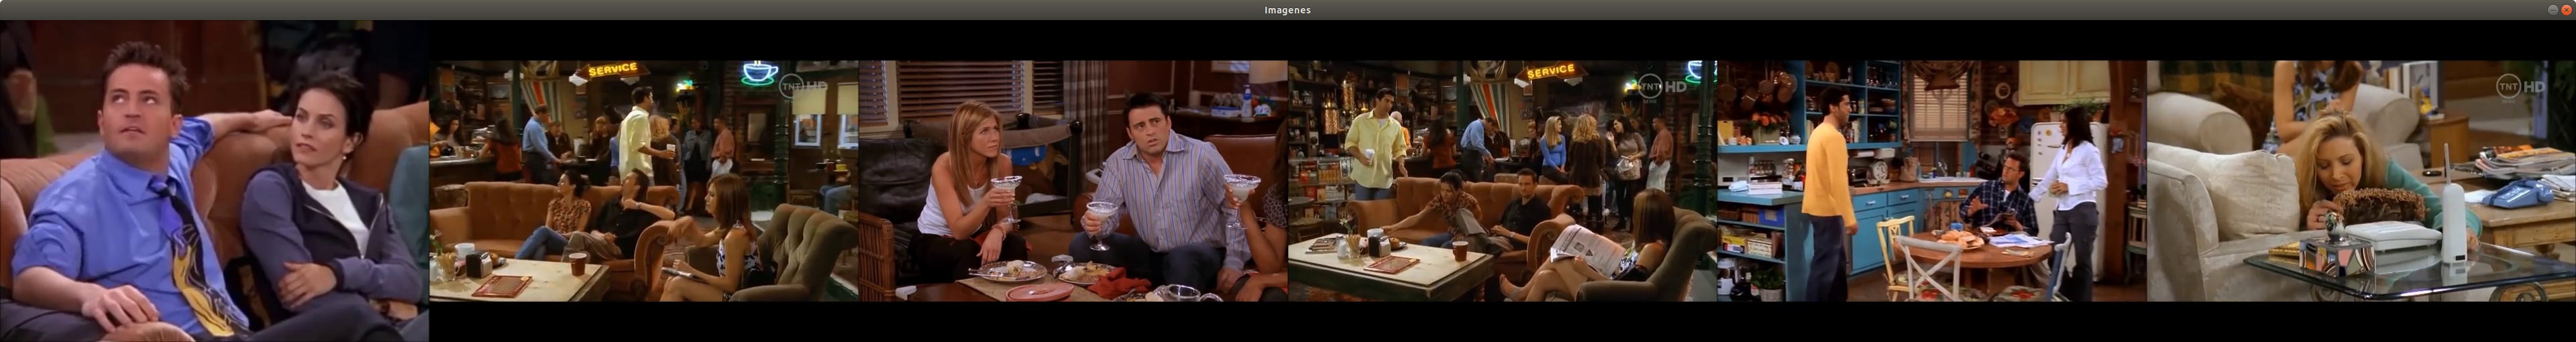
\includegraphics[scale=0.135]{./Imagenes/Ejercicio2-1.png}
  \caption{Imagen pregunta 15}
	\label{Ejercicio2-1}
\end{figure}

\begin{figure}[H]
  \centering
  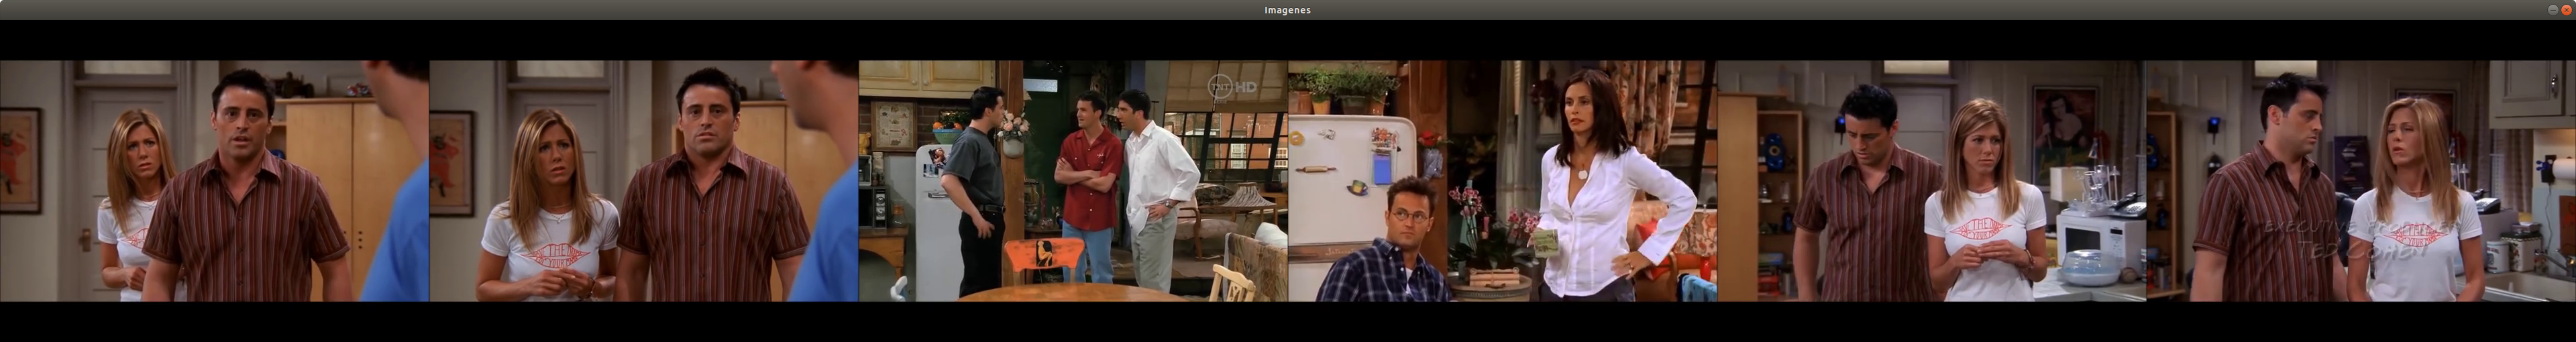
\includegraphics[scale=0.135]{./Imagenes/Ejercicio2-2.png}
  \caption{Imagen pregunta 209}
	\label{Ejercicio2-2}
\end{figure}

\begin{figure}[H]
  \centering
  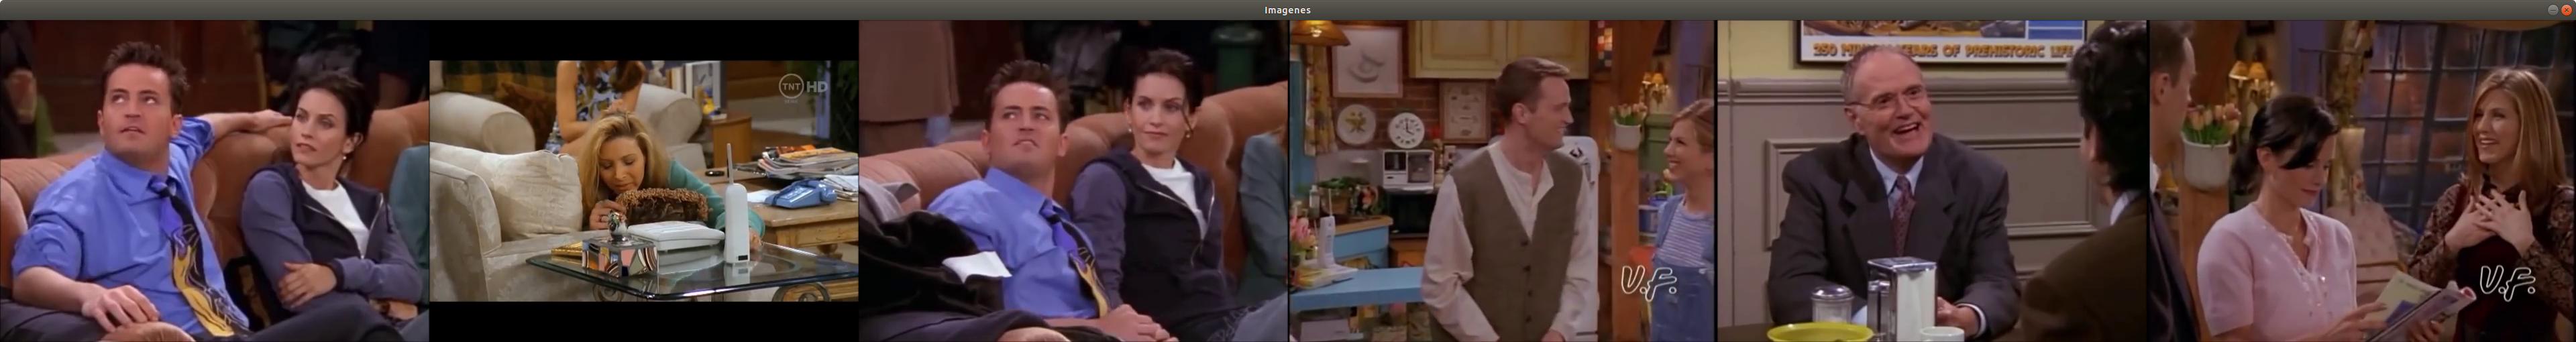
\includegraphics[scale=0.135]{./Imagenes/Ejercicio2-3.png}
  \caption{Imagen pregunta 1}
	\label{Ejercicio2-3}
\end{figure}

\begin{figure}[H]
  \centering
  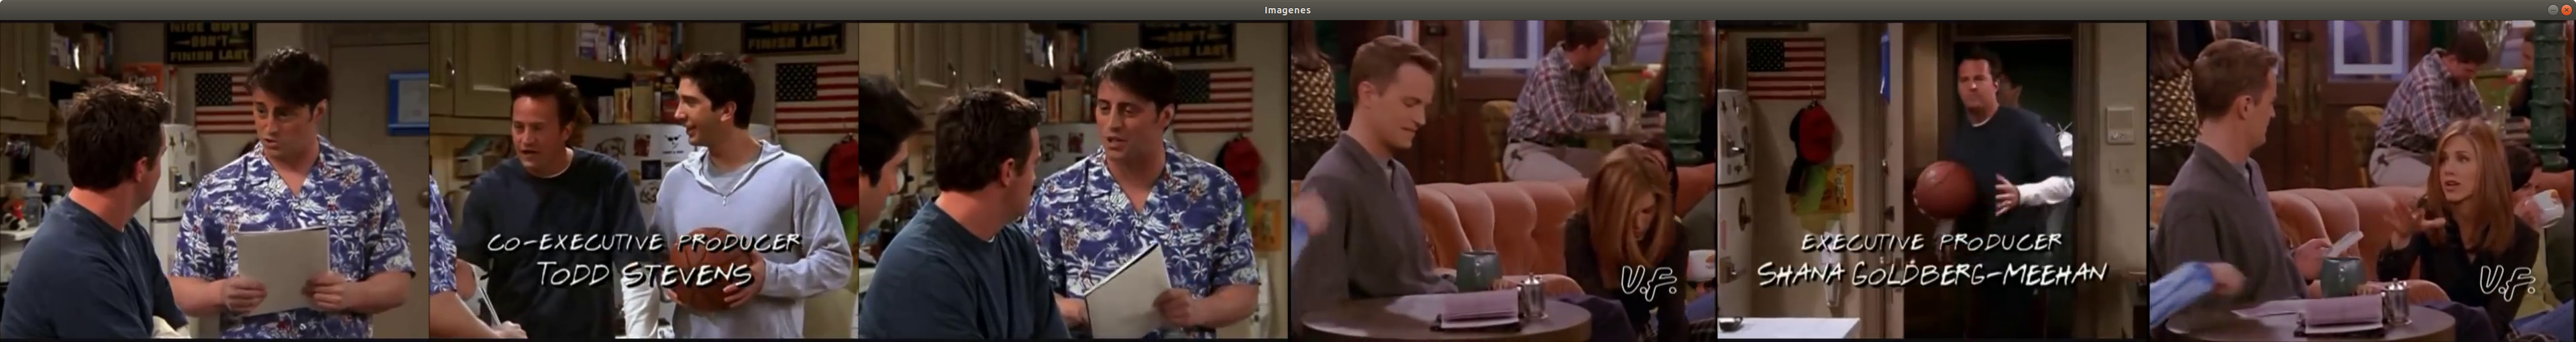
\includegraphics[scale=0.135]{./Imagenes/Ejercicio2-4.png}
  \caption{Imagen pregunta 91}
	\label{Ejercicio2-4}
\end{figure}

\begin{figure}[H]
  \centering
  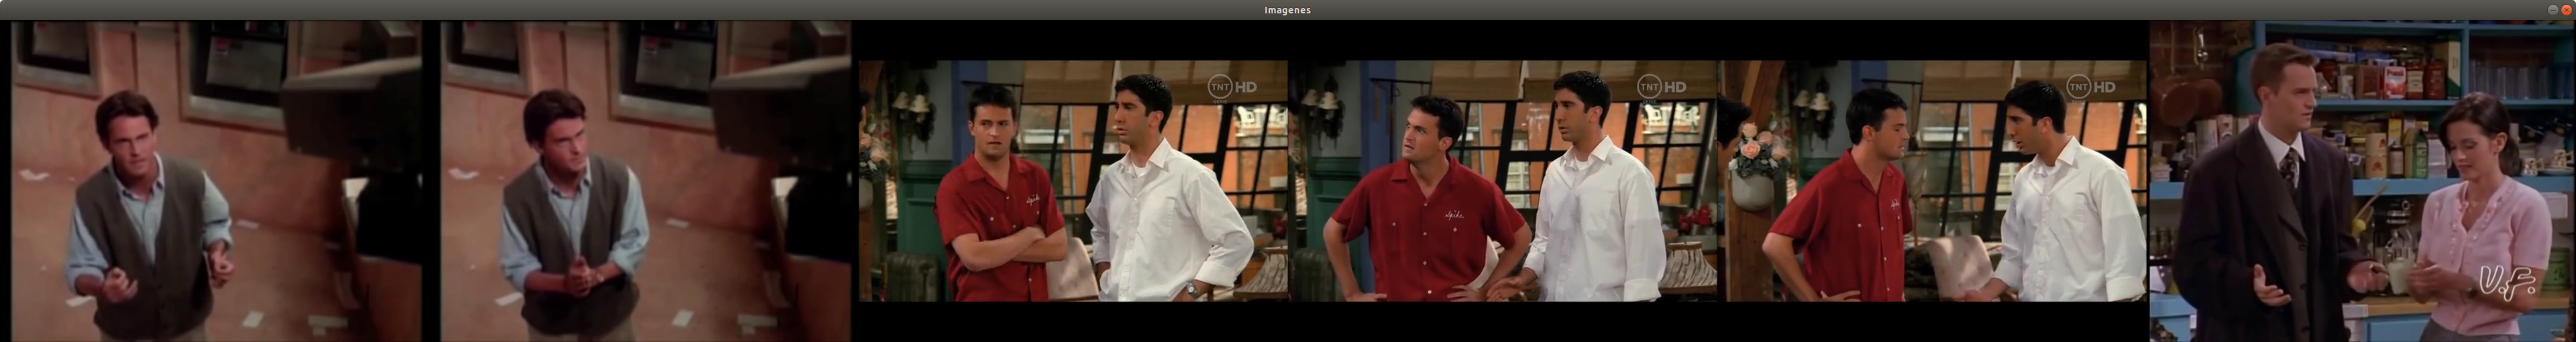
\includegraphics[scale=0.135]{./Imagenes/Ejercicio2-5.png}
  \caption{Imagen pregunta 200}
	\label{Ejercicio2-5}
\end{figure}

En estas imágenes cabe destacar que la primera de la tira es la propia imagen-pregunta y las 5 restantes son las emparejadas con la misma.

\vspace{10px}

Si observamos los resultados tenemos por ejemplo la imagen \ref{Ejercicio2-1} en la que las 5 imágenes obtenidas con más similitud son casi iguales, es decir, el emparejamiento es muy bueno. Si observamos el segundo de los casos en la imagen \ref{Ejercicio2-2} vemos que acierta en 3 de las 5 imágenes que ha tomado como las más similares y por tanto el resultado es bueno también. Si continuamos observando ya podemos percibir que en el reso de los casos el emparejamiento no es nada bueno como por ejemplo en las imágenes \ref{Ejercicio2-3} y \ref{Ejercicio2-4} en las que acierta en una o dos imágenes de las similares y por último el caso de la imagen \ref{Ejercicio2-5} en el que sólo la primera de las imágenes similares tiene algún parecido con la imagen-pregunta.

\vspace{10px}

Si analizamos más profundamente por qué hemos obtenido estos resultados podemos ver que, si tenemos imágenes con los mismos personajes, vestidos de igual forma y con un fondo igual o parecido entonces la similitud es muy alta. Si por contra por ejemplo tenemos a un mismo personaje con la misma ropa pero con dos fondos radicalmente diferentes como por ejemplo la imagen 208:

\begin{figure}[H]
  \centering
  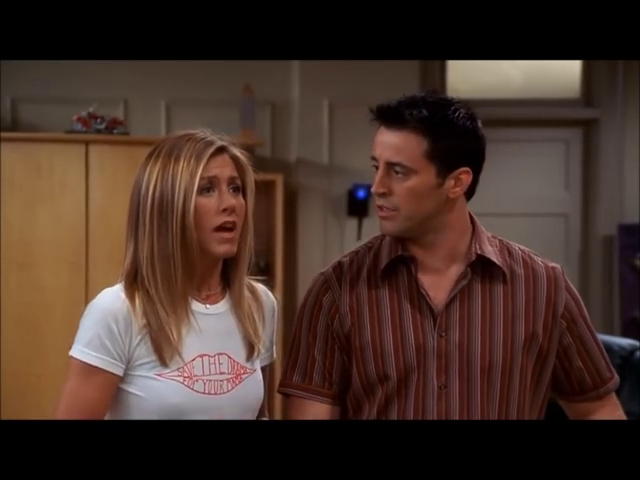
\includegraphics[scale=0.35]{./Imagenes/208.png}
  \caption{Imagen 208}
	\label{208}
\end{figure}

Esta imagen es claramente parecida a las que corresponden a la tira de imágenes \ref{Ejercicio2-2}, pero como podemos ver el fondo de esta imagen es radicalmente diferente al de la imagen pregunta, por lo que, aún siendo una foto que pertenece a la misma escena y debería ser de las más similares con respecto a la imagen-pregunta, no la estamos detectando como tal.

\vspace{10px}

Las conclusiones que podemos obtener de este experimento es que los resultados que obtengamos en cuanto a imágenes similares son altamente dependientes del número de descriptores obtenidos y de que las imágenes compartan un fondo parecido y unas figuras similares, si alguno de estos dos hechos varía entonces no obtendremos la similitud que buscamos. Esto es, si tenemos una imagen con un fondo similar pero con personajes distintos entonces no serán similares según este modelo y distancia o si tenemos imágenes con figuras similares o iguales pero un fondo diferente tampoco detectaremos a estas imagenes.

\section{Ejercicio 3}
Visualización del vocabulario
\begin{itemize}
  \item Usando las imágenes dadas en imagenesIR.rar se han extraído 600 regiones de cada imagen de forma directa y se han re-escalado en parches de 24x24 píxeles. A partir de ellas se ha contruido un vocabulario de 5000 palabras usando k-means. Los ficheros con los datos son descriptorsAndpatches2000.pkl (descriptores de las regiones y los parches extraídos) y kmeanscenters2000.pkl  (vocabulario extraído).
  \item Elegir al menos dos palabras visuales diferentes y visualizar las regiones imagen de los 10 parches más cercanos de cada palabra visual, de forma que se muestre el contenido visual que codifican (mejor en niveles de gris)
  \item Explicar si lo que se ha obtenido es realmente lo esperado en términos de cercanía visual de los parches.
\end{itemize}

\subsection*{\underline{Solución}}

Para resolver esto he desarrollado una función que toma los descriptores y parches del fichero descriptorsAndpatches2000.pkl y los centroides de kmeanscenters2000.pkl. Para cada centroide vemos cuales son los 10 descriptores de descriptorsAndpatches2000.pkl que están más cerca y tomamos sus regiones asociadas. De esta forma para cada uno de los centroides tendremos 10 regiones asociadas de mínima distancia. Ahora ordenamos este emparejamiento según la media de las distancias, esto es, obtendremos esta lista de centroides y parches ordenadas según distancia media de menor a mayor. De esta forma vamos a obtener en la primera posición los 10 parches asociados a un descriptor cuya distancia media es mínima en nuestro conjunto.

\vspace{10px}

Para obtener un resultado global e interpretable tomamos no sólo los elementos de mínima distancia si no también el de máxima distancia. Observemos los parches de los 3 primeros centroides con distancia mínima:

\begin{figure}[H]
  \centering
  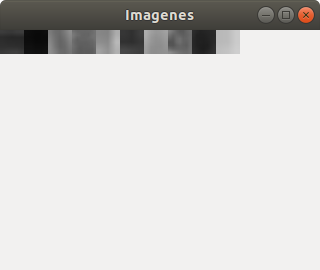
\includegraphics[scale=1.1]{./Imagenes/Ejercicio3-1.png}
  \caption{Parches del centroide de mínima distancia}
	\label{Ejercicio3-1}
\end{figure}

\begin{figure}[H]
  \centering
  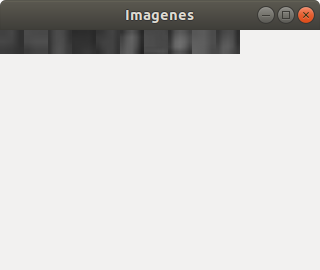
\includegraphics[scale=1.1]{./Imagenes/Ejercicio3-2.png}
  \caption{Parches del segundo centroide de mínima distancia}
	\label{Ejercicio3-2}
\end{figure}

\begin{figure}[H]
  \centering
  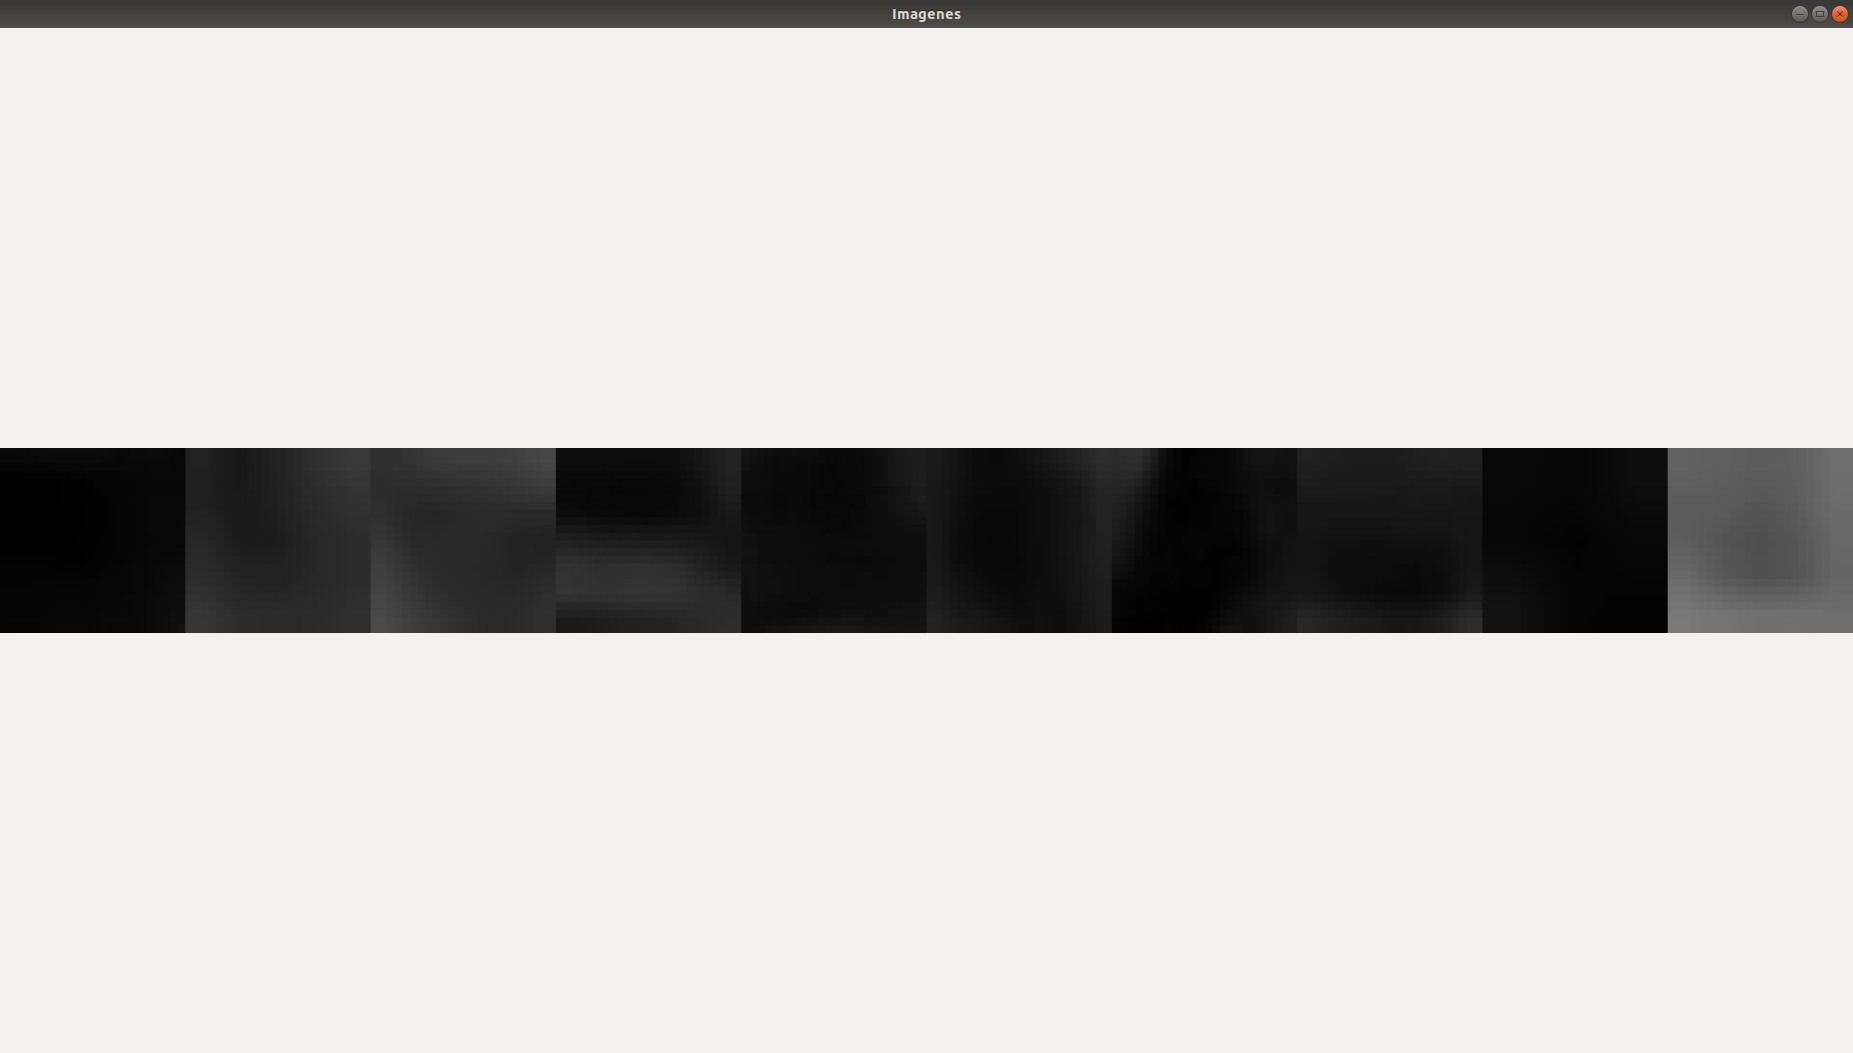
\includegraphics[scale=1.1]{./Imagenes/Ejercicio3-3.png}
  \caption{Parches del tercer centroide de mínima distancia}
	\label{Ejercicio3-3}
\end{figure}

Como podemos observar estos son los 3 conjuntos de 10 parches más parecidos entre sí. Si los observamos vemos que realmente tienen un parecido. Como mucho podríamos citar que en la segunda y tercera tira hay un elemento en el centro y al final respectivamente que destacan como bastante diferentes con respecto al resto, pero por el resto de imágenes no encontramos una diferencia muy grande.

\vspace{10px}

Observemos ahora el cconjunto de 10 parches con mayor distancia entre ellos.

\begin{figure}[H]
  \centering
  
\includegraphics[scale=1.1]{./Imagenes/Ejercicio3-4.png}
  \caption{Parches del centroide de máxima distancia distancia}
	\label{Ejercicio3-4}
\end{figure}

Estos 10 parches son los que mayor distancia media tienen entre sí. Como podemos ver realmente no hay una diferencia entre ellos enorme Quizás esta tira ha sido penalizada más en cuanto a la distancia porque alterna imágenes más claras y oscuras que en el resto (con tonos de gris claro más pronunciados y negros más pronunciados que el resto de imágenes). Aún así podemos ver que los parches escogidos no se diferencian entre sí al enlazarlos según el vocabulario que hemos obtenido.

\vspace{10px}

Este hecho no puede decirnos más que para los parches escogidos el vocabulario funciona razonablemente bien, lo que no quiere decir que si cambiásemos el conjunto de parches entonces seguiría funcionando igual de bien.

\end{document}
